\documentclass[12pt, twoside]{article}
\documentclass[12pt, twoside]{article}
\usepackage[letterpaper, margin=1in, headsep=0.2in]{geometry}
\setlength{\headheight}{0.6in}
%\usepackage[english]{babel}
\usepackage[utf8]{inputenc}
\usepackage{microtype}
\usepackage{amsmath}
\usepackage{amssymb}
%\usepackage{amsfonts}
\usepackage{siunitx} %units in math. eg 20\milli\meter
\usepackage{yhmath} % for arcs, overparenth command
\usepackage{tikz} %graphics
\usetikzlibrary{quotes, angles}
\usepackage{graphicx} %consider setting \graphicspath{{images/}}
\usepackage{parskip} %no paragraph indent
\usepackage{enumitem}
\usepackage{multicol}
\usepackage{venndiagram}

\usepackage{fancyhdr}
\pagestyle{fancy}
\fancyhf{}
\renewcommand{\headrulewidth}{0pt} % disable the underline of the header
\raggedbottom
\hfuzz=2mm %suppresses overfull box warnings

\usepackage{hyperref}
\usepackage{float}

\usepackage{pgfplots}
\pgfplotsset{width=9cm,compat=1.9}

\fancyhead[LE]{\thepage}
\fancyhead[RO]{\thepage \\ Name: \hspace{4cm} \,\\}
\fancyhead[LO]{BECA / Dr. Huson / Modeling \& Mathematics Applications\\* Quantifying Uncertainty: Probability \\* 4 March 2024}

\begin{document}
\begin{enumerate}
\subsubsection*{1.23 Exam: Probability, Venn diagrams}
\item Given: \\*
    $U = \{\text{the letters in the alphabet}\}$ \qquad
    $A = \{s, o, u, t, h\}$ \qquad
    $B = \{b, r, o, n, x\}$
    \begin{enumerate}[itemsep=1cm]
        \item List the members of $A \cap B$. \hfill [1 mark]
        \item List the elements of $A \cup B$. \hfill [1 mark]
        \item A letter of the alphabet is selected at random. What is the probability that it is a member of either or both sets, ($A \cup B$)? \hfill [1 mark]
    \end{enumerate} \vspace{1.5cm}

\item Events $A$ and $B$ are independent with $\mathrm P(A)=0.8$, $\mathrm P(B)=0.25$. Find each probability.
    \begin{enumerate}[itemsep=0.8cm]
        \item $\mathrm P(A \cap B)$ \hfill [2 mark]
        \item $\mathrm P(A \cup B)$ \hfill [2 mark]
        \item $\mathrm P(A \cap B')$ \hfill [2 mark]
        \item $\mathrm P(B | A)$ \hfill [2 mark]
        \item Mark the Venn diagram with the probabilities for each area. \hfill [2 marks]
    \end{enumerate}
    \begin{center}
        \begin{venndiagram2sets}[tikzoptions={scale=1.75}]
        \end{venndiagram2sets}U
    \end{center}


\newpage
\item The universal set $U$ is defined as the set of positive integers less than 9.
    \begin{enumerate}[itemsep=1.2cm]
        \item Subset is defined as $A =$ \{multiples of two\}. List its elements.  \hfill [1 mark] 
        \item Subset  $B =$ \{prime numbers\}. List the members of set $B$.  \hfill [1 mark]
        \item Place the elements of $U$ in the appropriate regions in the Venn diagram. \hfill [2 marks]
        \begin{center}
            \begin{venndiagram2sets}[tikzoptions={scale=2}]
            \end{venndiagram2sets}U
        \end{center}
        \item List the members of $(A' \cap B)$.  \hfill [1 mark]
        \item If an element of $U$ is selected at random, what is the probability that it is a member of both sets, ($A \cap B$)? \hfill [1 mark]
        \item If a member of set $A$ is selected at random, what is the probability that it is also a member of set $B$, i.e. the conditional probability ($B | A$)? \hfill [2 marks]
    \end{enumerate}

\newpage
\item A jar contains 20 marbles, 12 of which are red, 5 are blue, and 3 are green.
    \begin{enumerate}[itemsep=1.5cm]
        \item A marble is selected at random. Find the probability it is \emph{not} red. \hfill [1 mark]
        \item The marble is replaced and a second marble is selected. Given that the second marble is not red, find the probability it is green. \hfill [1 mark]
        \item The marbles are returned to the jar and two marbles are selected at random. Find the probability that both are blue. \hfill [2 mark]
    \end{enumerate} \vspace{1.5cm}

\item Draw a tree diagram to represent the taxi cab problem in the textbook. First, there are two cab companies, 85\% are black and the rest are yellow. Then, the witness identifies the color of the cab correctly 80\% of the time. \hfill [3 marks]
\begin{enumerate}
    \item Label the branches with the probabilities. \hfill [1 marks]
    \item Calculate the probabilities of each four outcomes. \hfill [2 marks]
    \item Given that the witness identified the cab as yellow, find the probability that it was black, i.e. that she was wrong. \hfill [3 marks]
\end{enumerate}

\newpage
\item \; \\
    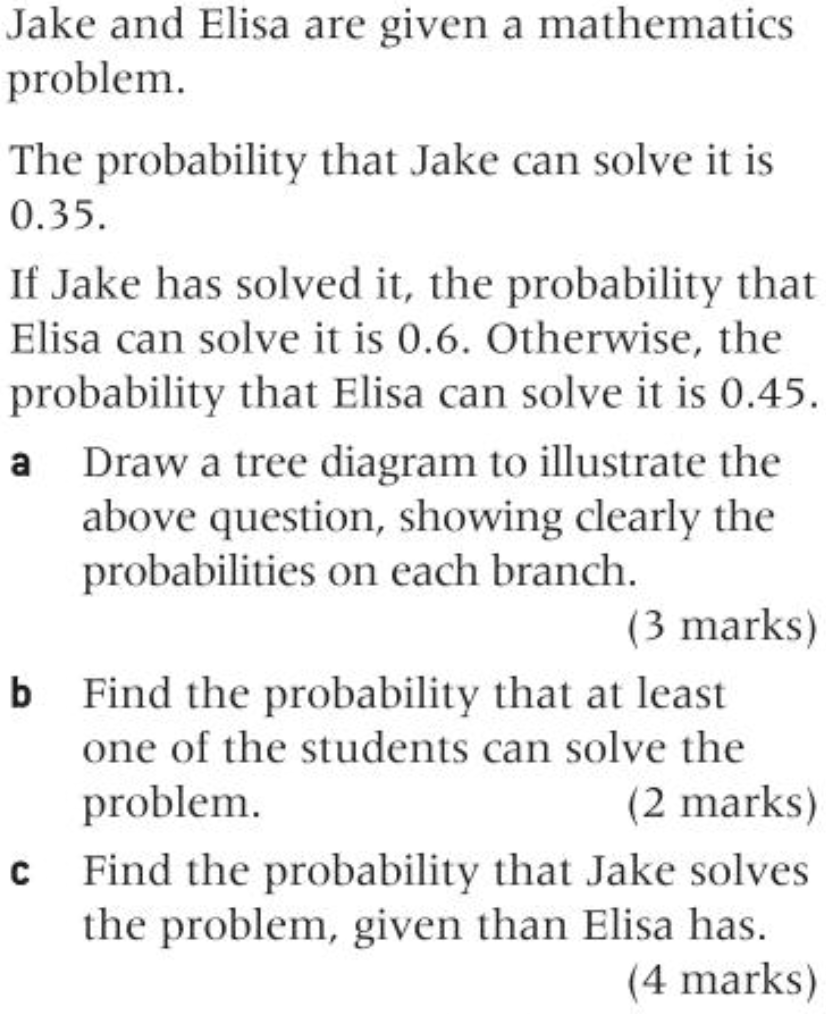
\includegraphics[scale=0.5]{../graphics/1-23Problem12-p374.png} \vspace{8cm}

\item The events $A$ and $B$ are mutually exclusive with $\mathrm P(A)=0.70$ and $\mathrm P(B)=0.2$.
    \begin{enumerate}[itemsep=1.5cm]
        \item Write down $\mathrm P(A \cup B)$. \hfill [1 mark]
        \item Write down $\mathrm P(A \cap B)$. \hfill [1 mark]
    \end{enumerate}

\newpage
\item Given events $A$ and $B$ with $\mathrm P(A)=0.7$, $\mathrm P(B)=0.5$, $\mathrm P(A \cap B)=0.35$.
    \begin{enumerate}
        \item Completely mark the Venn diagram with probabilities for each area. \hfill [2 marks]
        \begin{center}
            \begin{venndiagram2sets}[tikzoptions={scale=1.5}]
            \end{venndiagram2sets}
        \end{center}
        \item Find $\mathrm P(A \cup B)$. \hfill [2 marks] \vspace{1.5cm}
        \item State whether events $A$ and $B$ are independent. Justify your answer. \hfill [3 marks] \vspace{2.5cm}
    \end{enumerate}

\item For each Venn diagram, write an expression representing the shaded area. \hfill [5 marks] 
    \begin{multicols*}{2}
    \begin{enumerate}
        \item 
        \begin{venndiagram2sets}
            \fillNotB
            %\fillB
        \end{venndiagram2sets}
        \item %\\*[15pt]
            \begin{venndiagram2sets}
            \fillANotB
            \end{venndiagram2sets}
        \item %\\*[15pt]
        \begin{venndiagram2sets}
            \fillACapB
        \end{venndiagram2sets}
        \item %\*[15pt]
            \begin{venndiagram3sets}
            \fillC
            \fillBCapA
            \end{venndiagram3sets}
    \end{enumerate}
    \end{multicols*}

\newpage
\item A survey of fruit lovers is taken, all of whom like at least one of the three fruits: apples, bananas, and cherries. The following information is gathered:
    \begin{itemize}
        \item 50 people like apples
        \item 40 like bananas
        \item 30 like cherries
        \item 25 like apples and bananas
        \item 20 like apples and cherries
        \item 15 like bananas and cherries
        \item 10 like all three fruits
    \end{itemize}
Complete the Venn diagram below with the number of individuals in each region to represent the situation. How many people in total were surveyed? \hfill [4 marks] 
    \vspace{1cm}
    \begin{center}
        \begin{venndiagram3sets}[tikzoptions={scale=2.5}]
        \end{venndiagram3sets}U
    \end{center}


\end{enumerate}
\end{document}